\section {Other consoles}
This chapter talks about the less known / small consoles that either had a
short lifespan or their sales where not significant enough to compete with
the major video game consoles previously exposed. These consoles are
drastically different and where produced in different years. The consoles:\\

\subsection{Atari 2600:}
The Atari 2600 (or Atari VCS before 1982) is a home video game console by
Atari, Inc. Released on September 11, 1977, The console was originally sold
as the Atari VCS, an abbreviation for Video Computer System. Following the
release of the Atari 5200 in 1982, the VCS was renamed to the "Atari 2600",
after the unit's Atari part number, CX2600. The 2600 was typically bundled
with two joystick controllers, a conjoined pair of paddle controllers, and a
game cartridge: initially Combat, and later Pac-Man\cite{Atari2600}. The
total games registered in the dataset for the Atari 2600 where 133 with total
sales for this platform for \$97.08 million dollars with its most
representative game being \textit{Pac-Man} released in 1982 with sales for
\$7.81 million dollars.

\subsection{Wonder Swan:}
The WonderSwan is a handheld game console released in Japan by Bandai. It was
developed by Gunpei Yokoi's company Koto Laboratory and Bandai. Released in
1999, the WonderSwan Color and SwanCrystal were officially supported until
being discontinued by Bandai in 2003. During its lifespan, no variation of
the WonderSwan was released outside Japan. It was Powered by a 16-bit central
processing unit, the WonderSwan took advantage of a low price point and long
battery life in comparison to its competition, Nintendo's Game Boy Color and
SNK's Neo Geo Pocket Color\cite{WonderSwan}. The dataset only contains 6
registered games for this platform with sales for \$1.42 million dollars; the
most representative game is \textit{Final Fantasy} released in 2000 making
half a million dollars.

\subsection{Neo Geo:}
 the Neo Geo MVS and its home console counterpart, the Neo Geo AES. Both the
 arcade system and console were powerful for the time and the AES allows for
 perfect compatibility of games released for the MVS. However, the high price
 point for both the AES console and its games prevented it from directly
 competing with its contemporaries, the Sega Mega Drive (Genesis), Super NES
 (Super Famicom), and Turbo-Grafx 16\cite{NeoGeo}.\\
 Its most representative game was \textit{Samurai Showdown II} released in
 1994 and making \$250.000 usd. The NeoGeo only has 12 registered games in the
 dataset and according to it, it produced \$1.44 million dollars on its
 lifespan.

 \subsection{Turbo Grafx 16:}
 The TurboGrafx-16 Entertainment SuperSystem, known in Japan and France as
 the PC Engine, is a home video game console jointly developed by Hudson Soft
 and NEC Home Electronics, released in Japan on October 30, 1987, in the
 United States on August 29, 1989, and in France on November 22, 1989. It was
 the first console released in the 16-bit era, albeit still utilizing an
 8-bit CPU. Originally intended to compete with the Nintendo Entertainment
 System (NES), it ended up competing with the Sega Genesis, and later on the
 Super Nintendo Entertainment System (SNES)\cite{TurboGrafx}.\\
 The Turbo Grafx only has 2 games registered in the dataset with total sales
 of 160.000usd.
 \subsection{3DO Interactive Multiplayer:}
 The 3DO Interactive Multiplayer, often called simply the 3DO, is a home
 video game console platform developed by The 3DO Company.The 3DO was not a
 console manufactured by the company itself, but a series of specifications,
 that could be licensed by third parties. Panasonic produced the first
 models in 1993, and further renditions of the hardware were released in 1994
 by Sanyo and GoldStar (now LG Corp).\\
 Despite a highly promoted launch (including being named Time magazine's
 "1993 Product of the Year") and a host of cutting-edge technologies, the
 3DO's high price and an oversaturated console market prevented the system
 from achieving success comparable to veteran competitors Sega and
 Nintendo. As a result, it was discontinued in late 1996, three years after
 its first release\cite{Panasonic3DO}.\\
 According to the dataset, the console only generated 100.000usd with 3
 registered games.

 \subsection{NEC PC-FX:}
 The PC-FX is a 32-bit home video game console made by NEC Home
 Electronics. It was released in Japan on December 23, 1994, just weeks after
 Sony's PlayStation and a month after the Sega Saturn. It is the successor to
 the PC Engine, known as TurboGrafx-16 in North America. PC-FX was only
 released in Japan. The console is shaped just like a tower PC and was meant
 to be similarly upgradeable. However the PC-FX was using an outdated
 graphics chip that rendered the system underpowered in comparison to its
 competitors, which caused it to be a commercial failure\cite{PCFX}. The PCFX only has 1
 registered game and according to the data it only sold 30.000usd.\newpage

To check with more detail the sales for these platforms just point
\textit{ARMeet} to Figure \ref{fig:OtherImage}.\\

\begin{figure}[h]
  \centering
  \centerline{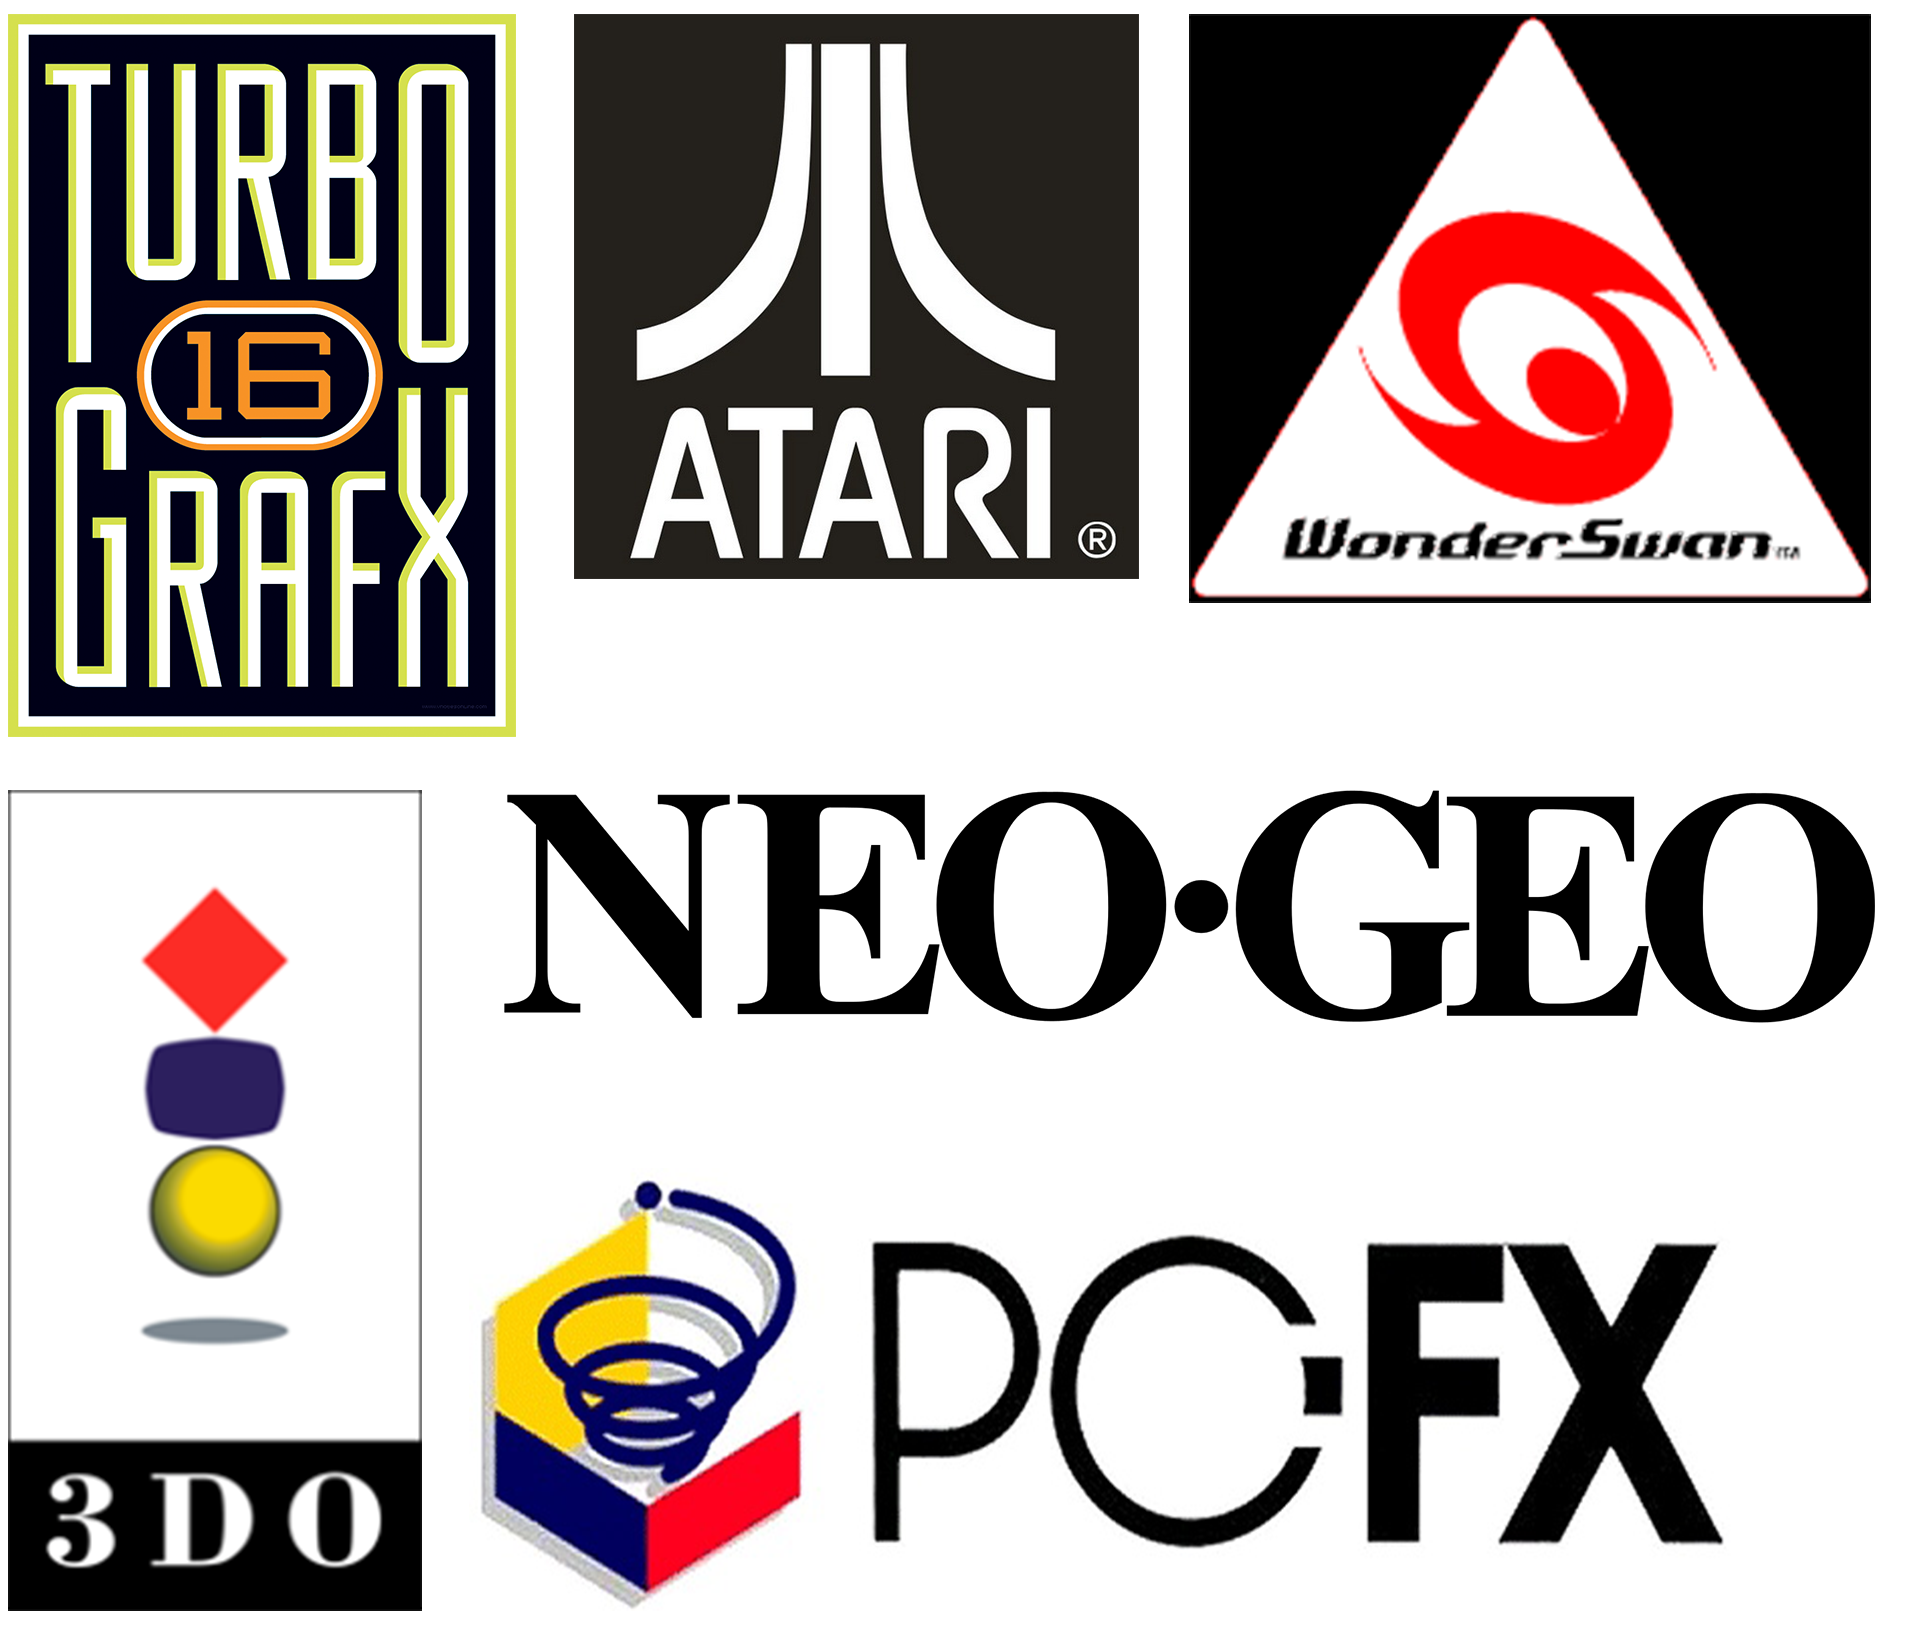
\includegraphics[scale=0.2]{images/OtherMainTarget.png}}
  \caption{Representative picture of all the other platforms, point ARMeet to this image to
    see the different sales on each platform.}
  \label{fig:OtherImage}
\end{figure}

%% Platform: ATARI2600
%% Games: 133
%% Total Sales: 97.07996, by country US: 90.60001 EU: 5.470006 JP: 0 Other: 0.9099996

%% Platform: TG16
%% Games: 2
%% Total Sales: 0.16, by country US: 0 EU: 0 JP: 0.16 Other: 0

%% Platform: NEO_GEO
%% Games: 12
%% Total Sales: 1.44, by country US: 0 EU: 0 JP: 1.44 Other: 0

%% Platform: _3DO
%% Games: 3
%% Total Sales: 0.09999999, by country US: 0 EU: 0 JP: 0.09999999 Other: 0

%% Platform: PCFX
%% Games: 1
%% Total Sales: 0.03, by country US: 0 EU: 0 JP: 0.03 Other: 0

%% Platform: WONDER_SWAN
%% Games: 6
%% Total Sales: 1.42, by country US: 0 EU: 0 JP: 1.42 Other: 0
